%%
%%                      Notes on Relational Theory
%%
%% License:
%%   Public Domain
%%
%% Author:
%%   Ahmed S. Darwish <darwish.07@gmail.com>, with excerpts from
%%   E. F. Codd's papers in the first section `The relational model'
%%
%% TODO:
%% - Recursive closure; rel. algebra recursive-infeasibility proof[*]
%% - Normalization and functional dependencies
%% - Soundness and completeness of Armstrong inference rules
%% - On an appendix: an SQL equivalent of algebraic queries given
%%
%% Evolution to the next version:
%% - Include commented-out 'INTEGRATE'-marked paragraphs
%% - Really use `multicol'
%% - Use a 10 or 11pt text font; the current one is huge
%% - proofread the overall final result
%%
%% Source-text coding style (line-feeds included):
%% - Paragraphs text <= 77 columns
%% - Math equations  <= 80 columns
%% - Comments        <= 70 columns
%%

\documentclass [a4paper, 12pt, twocolumn]{article}

\addtolength{\textwidth}{50pt}
\addtolength{\evensidemargin}{-25pt}
\addtolength{\oddsidemargin}{-25pt}

\usepackage{amsmath}                    % multi-line equations
\usepackage{verbatim}                   % multi-line comments
\usepackage{multicol}                   % multi-column the title!
\usepackage{wasysym}                    % relational '\Join'

\usepackage{graphicx}                   % include graphics
\graphicspath{{graphs/}}                % graphicx: figures search path

\usepackage[                            % tables and figures caption style:
  small,                                % ..small font
  labelformat=parens,                   % ..ala parens @ 'Figure (2)'
  labelfont=bf,                         % ..bold the 'Figure (1)' part
  textfont=it]{caption}                 % ..italicize description font

\newcommand{\db}   {\displaybreak[0]}   % break multi-line math over pages
\newcommand{\m}    {\mathit}            % mathify big variable names
\newcommand{\band} {\ \textbf{and}\ }   % bold 'and' for selection conditions
\newcommand{\bor}  {\ \textbf{or}\ }    % bold 'or' for selection conditions
\newcommand{\<}    {\langle}            % '<', not treated as an operator
\renewcommand{\>}  {\rangle}            % '<', not treated as an operator
\newcommand{\lar}  {\leftarrow}         % assignment operator shorthand
\newcommand{\q}    {\quad}              % 4 programmed spaces
\newcommand{\qq}   {\qquad}             % 8 programmed spaces
\newcommand{\thet} {\ \theta\ }

%%
%% For breaking multi-line equations across pages, check
%% \displaybreak[0] and \allowdisplaybreaks from AMS official docs se-
%% ction3.9: 'Vertical spacing and page breaks in multiline displays'.
%%

\begin{document}

\title{Notes on Relational Theory}

\author{Ahmed S. Darwish\footnote{These notes are based on the databases book
cited at \cite{elmasri}. Excerpts from E. F. Codd's papers are included in the
first section.}\\
\texttt{darwish.07@gmail.com}}

\maketitle

\subsection{The relational model}

The relational model stresses on \emph{separation of concerns} by means
of data independence: application programs should not be logically impaired
cause of growth in data types and changes in data representation. It provides
means to describe data in its natural structure only, without imposing
\emph{any} additional structure for machine representation.\cite{codd-v1}

This data model central concept is the \emph{relation} in its mathematical
set theory sense. Relations were informally described by De Morgain as
\begin{quote}
When two objects, qualities, classes, or attributes, viewed together by the
mind, are seen under some connexion, that connexion is called a relation.
\end{quote}
where an example is the fatherhood relation between a person-male father, and
a person child whether male or female. Such a relation can be represented as
$\m{F}$ $=$ $\{\<\m{Adam}$, $\m{Jane}\>$, $\<\m{Adam}$, $\m{Casey}\>$,
$\ldots \}$ where $\<X, Y\>$ $\in$ $\m{F}$ implies person $X$ as a father of
$Y$ in the miniworld the relation represents.

Mathematically, given sets $S_1, S_2, \ldots, S_n$ representing domains that
are not necessarily distinct, $R$ is called a relation on these $n$ sets if
it is a set of $n$-tuples\footnote{An $n$-tuple is an ordered list of $n$
elements.} each of which has its first element from $S_1$, its second element
from $S_2$, and so on. More concisely:
\begin{equation*}
  R \subseteq S_1 \times S_2 \times \ldots \times S_n
\end{equation*}
where $S_j$ is referred as the $j$th domain of $R$, and `$\times$' is the
cartesian product operator.

Relations are sets, but not all sets are relations. The elements of a
relation of degree $n$ are called $n$-tuples or tuples. A relation $R$ has
the following properties: (1) each row represents an $n$-tuple of R, (2) the
ordering of rows is insignificant, (3) rows are distinct, (4) the ordering of
columns is significant cause it corresponds to the ordering
$S_1, S_2, \ldots, S_n$ of the domains\footnote{This property has been
relaxed in further iterations of the model by mandating a distinct (column)
name for each participating domain role.}. Denoting $|X|$ as the number of
elements in set $X$, we have:
\begin{equation*}
  |R| \le |S_1| * |S_2| * \ldots * |S_n|
\end{equation*}

One domain (or combination of domains) of a given relation has values which
uniquely identify each $n$-tuple element of that relation. Such a domain (or
a combination) is called the \emph{primary key}. A domain (or a domain
combination) of relation $R$ is a \emph{foreign key} if it's not the primary
key of $R$ but its elements are values of the primary key of some relation
$S$, where the possibility of $S \equiv R$ is not excluded.

The domain elements are \emph{atomic} (nondecomposable) values within the
system data model. A relation is in its \emph{first normal form} if it has
the property that none of its domains has elements which are themselves sets.
An \emph{unnormalized relation} is one which is not in its first normal form.
The first normal form is sometimes called the \emph{flat relational model};
much of the relational model theory was developed with this flat model in
mind.

Further notation was eventually added to the relational model. A
\emph{relation schema} $R(A_1, A_2, \ldots, A_n)$ is made-up of relation name
$R$ and the list of attributes $A_1, \ldots, A_n$, where each attribute is a
name of a \emph{role}\footnote{The \emph{role} concept was originally created
by Codd to distinguish equivalent domains in the same relation.} describing a
relation-participating domain set. A relation instance $r(R)$ is one of the
possible $n$-tuples sets $r(R) = \{t_1, t_2, \ldots, t_m\}$ materializing the
relation schema definition $R$. A value in tuple $t \in r(R)$, corresponding
to an $R$'s attribute $A$ (or a combination), can be referred to as
$t[A]$.\footnote{For simplicity, the \emph{notational} difference between a
schema $R$ and its instance $r(R)$ is sometimes ignored.}

There can be many \emph{constraints} on the data-model imposed by the
miniworld the database represents. \emph{Domain constraints} specify that
corresponding values for each attribute $A$ must be an atomic element from
the domain set: $\forall t \in r(R) \colon t[A] \in \m{dom}(A)$. The
\emph{key constraint} mandates that for any superkey subset of attributes
$\m{SK}$, we have $\forall
t_i \in r(R), t_j \in r(R), i \not= j \colon t_i[\m{SK}] \not= t_j[\m{SK}]$.
Another constraint is the \emph{not-null constraint} where some attributes
are not allowed to have undefined (\verb/NULL/) values.\cite{elmasri}

Since no positional identification of tuples exists, the
\emph{entity-integrity constraint} mandates that primary key values cannot be
\verb/NULL/: it would imply an inability to identify some tuples. Finally,
the \emph{referential integrity constraint} is used to maintain consistency
among two relations tuples. A set of attributes $\m{FK}$ in the relation $R$
is a valid foreign key to relation $S$ if (1) the attributes in $\m{FK}$ have
the same domain as the primary key attributes $\m{PK}$ of $S$, and (2)
$\forall t_i \in r(R) \colon
t_i[\m{FK}] = \hbox{\verb/NULL/} \lor
\exists t_j \in s(S) \colon t_i[\m{FK}] = t_j[\m{PK}]$.

%%% ** INTEGRATE ** %%%
\begin{comment}

``Consider for example a data bank which contains information about parts,
projects, and suppliers. The individual description for an individual object
(such as a particular part) is called an \emph{entity}. The prototype
description for a class of objects is called an \emph{entity-type}. The set
of entities of a given entity type can be viewed as a relation, and we shall
call it an entity-type relation.
...
The remaining relations in a data bank are between entity types, are are
therefore called inter-entity relations. An essential property of every
inter-entity relation is that its domains include at least two keys which
either refer to two distinct entity-types or refer to a common entity type
serving distinct roles.''       -- E.F. Codd, RJ599 IBM research report

Defining \emph{entity} as the individual description of an individual object
(e.g., a particular employee) and an \emph{entity type} as a prototype
description for a class of objects (e.g. common traits needed to describe
an employee in the represented miniworld), the ``set of entities for a given
entity type'' can be viewed as a relation. Such a relation was referred to as
an \emph{entity type relation} in Codd's very first paper on the relational
model.\cite{codd-v0} Figure~(\ref{fig:schema})'s entity type relations are
the `Employee', `Department', `Project', and `Dependent' ones.

The remaining relations in a database are between entity types, and were thus
called \emph{inter-entity relations}. Every inter-entity relation includes at
least \emph{two} foreign keys which either refer to two distinct entity-types
or refer to a common entity-type serving distinct roles (e.g. a supervisor
and a supervisee role played by entities in the same `employee' entity type).
Figure~(\ref{fig:schema})'s inter-entity relations are the `Works\_on' and
`Dept\_locations' ones. Interestingly, this semantic interpretation of the
relational model existed long before the entity-relationship approach was
being published and publicized as an extended
``data model''.\cite{date-introduction}

\bibitem{codd-v0}
  E. F. Codd,
  \emph{Derivability, Redundancy and Consistency of Relations Stored in
    Large Data Banks}.
  IBM Research Report RJ599, San Jose, California, August 1969.

\bibitem{date-introduction}
 C. J. Date,
 \emph{An Introduction to Database Systems -- 8\textsuperscript{th} Edition}.
 Addison-Wesley, 2004.

\end{comment}

Finally, note that the terms ``relation'' and ``table'' are not synonymous.
From their set bases, relations have no positional concepts. Thus, there's
no ``nextness'' of rows. Similarly, and especially in later versions of the
model, one may shuffle the columns without affecting the information content,
providing the column heading is taken with each column. Thus, there's also no
``nextness'' of columns. Neither of these activities can occur with such
immunity to arrays.\cite{codd-v2}

\subsection{Relational algebra}
Beside the regular set theory operators, the relational algebra operators are
introduced because of their key role in deriving relations from other
relations. \emph{Selection}: filter tuples that satisfies a certain
condition. It can be visualized as a \emph{horizontal partitioning} between
two set of tuples, those tuples that satisfy the condition, and those that do
not:
  \[\sigma_{<selection\_condition>}(R)\]
where $\<$selection\_condition$\>$ = $\<$attribute\_name $A\>$
$\<$comparison op$\>$ $\<$value $\in dom(A) \>$ or
$\<$selection\_condition$\>$ = $\<$attribute\_name $A_i\>$
$\<$comparison op$\>$ $\<$attribute\_name $A_j\>$ where
$\m{dom}(A_i) = \m{dom}(A_j)$. From definition, some of the selection
operator properties include:
\begin{flalign*}
  &\q\sigma_{<c1>}(\sigma_{<c2>}(R)) = \sigma_{<c1 \band c2>}(R) &\\
  &\q\sigma_{<c1>}(\sigma_{<c2>}(\ldots(\sigma_{<cn>}(R))\ldots)) &\\
  &\q\qquad \equiv \sigma_{<c1 \band c2 \band \ldots \band cn>}(R) &\\
  &\q\sigma_{<c1>}(\sigma_{<c2>}(R)) = \sigma_{<c2>}(\sigma_{<c1>}(R)) &\\
  &\q|\sigma_{<c>}(R)| \le |R| &
\end{flalign*}

\emph{Projection}: selects certain columns of the relation (striking out the
others), then removes from the resulting array any duplication of rows. The
final array represents a relation which is said to be a projection of the
given relation. This operator can be visualized as a \emph{vertical
partitioning} of the relation into two instances: one that does include the
specified attributes, and another that does not:
  \[\pi_{<attribute\_list>}(R)\]
where $\<$attribute\_list$\>$ is the desired list of attributes from relation
$R$. If any attribute is in $\langle$attribute\_list$\rangle$ but not in $R$,
then the expression is incorrect. Some properties include:
\begin{flalign*}
  &\q\pi_{<list1>}(\pi_{<list2>}(R)) = \pi_{<list1>}(R) &\\
  &\q\pi_{<A1, A2, \ldots, An>}(\sigma_c(R)) =
    \sigma_c(\pi_{<A1, A2, \ldots, An>}(R)) &
\end{flalign*}
where $\<$list1$\>$ includes \emph{all} the $\<$list2$\>$ attributes and the
selection condition $c$ involves \emph{only} attributes from the set
$\{A_1, A_2, \ldots, A_n\}$.

\emph{Set operators}: relations are sets, thus all of the usual set
operations are applicable. Nevertheless, the result may \emph{not} be a
relation: for example, the union of a binary relation and a ternary relation
is not one. Two relations $R(A_1$, $A_2$, $\ldots$, $A_n)$ and $S(B_1$, $B_2$,
$\ldots$, $B_m)$ are \emph{union-compatible} if they have the same degree
($n = m$) and if $dom(A_i) = dom(B_i)$ for all $1 \le i \le n$.\footnote{To
let the set operators result in a relation, the result set -- as in any
relation -- must be totally built from the same type of tuples. Two tuples
are of the same type if they have the same length and include equivalent
domains for each corresponding tuple attribute.} Some of the set operators
properties include:
\begin{flalign*}
  &\q R \cup S = S \cup R, \ \hbox{and}\  R \cap S = S \cap R&\\
  &\q R - S \not= S - R &\\
  &\q\sigma_c(R \thet S) = \sigma_c(R) \thet \sigma_c(S) &\db\\
  &\q\pi_L(R \cup S) = \pi_L(R) \cup \pi_L(S) &
\end{flalign*}
where $\theta$ is any of the set operators $\cup$, $\cap$, or
$-$. Finally, note that projection can't be commuted with intersection or set
difference (`$\cap$', `$-$') since it conflicts with these operators
\emph{column-sensitive} semantics.

%% The cartesian product _can_ be useful on its own as shown in Orielly's
%% 'Learning SQL' book, chapter 10 'Joins Revisited', 10.2 'Cross Joins'.
\emph{Cartesian Product}: the well-known set-theory operator used to combine
every member from the first set with every member from the second set; it
can be used between relations which are \emph{not} union compatible.
Given $R(A_1$, $A_2$, $\ldots$, $A_n)$ and $S(B_1$, $B_2$, $\ldots$, $B_m)$,
we have $Q(A_1$, $A_2$, $\ldots$, $A_n$, $B_1$, $B_2$, $\ldots$, $B_m)$ of
degree $n + m$ if $R \times S = Q$. Assuming $|R| = n_r$ and $|S| = n_s$,
then $|Q| = n_r * n_s$. In general, the cartesian product is not very useful
on its own, but by using selection afterwards, it can be exploited to select
matching tuples from \emph{any} two relations.

Some properties include: (1) if the selection condition $c$ only involves
attributes of $R$, we have $\sigma_c(R \times S) = \sigma_c(R) \times S$, (2)
alternatively, if the condition $c$ can be written as
$(c_1 \small{\band} c_2)$ where condition $c_1$ only involves attributes from
$R$ and $c_2$ only involves attributes from $S$, we have:
\begin{flalign*}
  &\q\sigma_{d}(R) \times \sigma_{e}(S) = \sigma_{<d \band e>}(R \times S)&\\
  &\q\sigma_c(R \times S) = \sigma_{c1}(R) \times \sigma_{c2}(S)&
\end{flalign*}
\begin{comment}
In the second equation above, if $c$ contains \emph{some} expressions that
forbid it from being formulated in the $c_1 \land c_2$ form, those offending
expressions can be added to an extra final selection on the far left of the
right hand side.
\end{comment}
where $d$ and $e$ are selection conditions, (3) commutativity with
projection: suppose $L = $ $\{A_1$, $\ldots$, $A_n$, $B_1$, $\ldots$, $B_m\}$
where $A_i$ is an attribute of $R$ and $B_j$ is an attribute of $S$ for all
$1 \le i \le n$ and $1 \le j \le m$, we have
$\pi_L(R \times S) \equiv \pi_{<A1,\ldots,An>}(R) \times
\pi_{<B1,\ldots,Bm>}(S)$.

\emph{Join}: one of the most important operators in relational algebra by
allowing us to exploit the implicit relationships between relations: it
combines related tuples from two relations into a single tuple. For
$R(A_1,\ldots,A_n)$ and $S(B_1,\ldots,B_m)$, we have the join $Q$ of degree
$n + m$:
  \[Q = R \Join_c S = \sigma_c(R \times S)\]
where condition $c$ contains expressions in the form $A_i \thet B_j$ for
$1 \le i \le n$ and $1 \le j \le m$, $dom(A_i) = dom(B_j)$, and
$\theta \in \{<$, $\le$, $=$, $>$, $\ge$, $\not=\}$.
Finally assuming $|R| = n_r$, and $|S| = n_s$, we have
$0 \le |Q| \le n_r * n_s$.\footnote{Compare this with cartesian product's
$|Q| = n_r * n_s$.} The referential integrity constraint is essential in
having matching tuples in the resulting relation.

Similar to the cartesian product, a selection with condition $c$ can be
commuted with the join `$R \Join_d S$' if $c$ can be expressed in the form
$c_1 \land c_2$, where $c_1$ only involves attributes from $R$ and $c_2$ only
contains attributes from $S$:
\begin{flalign*}
  &\q\sigma_c(R \Join_d S) &\\
  &\q\q= \sigma_c(\sigma_d(R \times S)) &\\
  &\q\q= \sigma_d(\sigma_c(R \times S)) &\\
  &\q\q= \sigma_d(\sigma_{c1}(R) \times \sigma_{c2}(S)) &\\
  &\q\q= \sigma_{c1}(R) \Join_d \sigma_{c2}(S) &
\end{flalign*}
by the join operator definition, commutativity of selection, and by commuting
`$\sigma$' with `$\times$'. Similarly, projection can be commuted with the
join: \begin{flalign*}
  &\q\pi_L(R \Join_d S) &\\
  &\q\q= \pi_L(\sigma_d(R \times S)) &\\
  &\q\q= \sigma_d(\pi_L(R \times S)) &(*)&\\
  &\q\q\equiv \sigma_d(\pi_{A1,\ldots,An}(R) \times \pi_{B1,\ldots,Bm}(S)) &\\
  &\q\q\equiv \pi_{A1,\ldots,An}(R) \Join_d \pi_{B1,\ldots,Bm}(S) &
\end{flalign*}
where the list of projection attributes
$L = \{A_1, \ldots, A_n, B_1, \ldots, B_m\}$ having $A_1, \ldots A_n$ as a
subset of $R$'s attributes and $B_1, \ldots, B_m$ as a subset of $S$'s
attributes, and where all attributes in the join condition $d$ are covered in
projection list $L$ due to the transformation line marked by $(*)$.

%%% ** INTEGRATE ** %%%
\begin{comment}

While comprehending some of the complex equations above, it's best to
visualize the set operators working on horizontal tuples while other
operators like $\pi$ work on vertical attributes, building a \emph{different}
set of horizontal tuples. Finally, remember that all relational algebraic
operators also produce a relation, satisfying the model's \emph{closure}
property and making the relational algebra a \emph{closed system}.

\end{comment}

\emph{Division}: the algebraic counterpart of predicate logic's
\emph{universal quantifier}.\cite{codd-semantic} Let $Z$, $X$, $Y$ be sets of
relation attributes where $X \subseteq Z$, $Y  = Z - X$, and thus
$Z = X \cup Y$. Letting $R(Z)$, $S(X)$, and $T(Y)$ be relations on these
attributes, we can define division as
\begin{equation} \label{div}
  T(Y) = R(Z) \div S(X)
\end{equation}
where:
\begin{flalign} \label{div2}
  &\q t_y \in T \Longleftrightarrow (S \times \{t_y\}) \subseteq R&
\end{flalign}
and $R = (S \times T) \cup D$, having $D$ as the division remainder. Note
that throughout this formalization, relations are considered
domain-unordered: a \emph{relationship}, using Codd's terminology. Thus, the
cartesian product results in equation (\ref{div2}) are only
\emph{semantically} union-compatible with $R$.

As a moderate example, let $R(a, b)$ $=$
$\{\<p, 1\>$, $\<p, 2\>$, $\<p, 3\>$, $\<q, 1\>$, $\<r, 1\>$, $\<r, 3\>\}$
and $S(b) =$ $\{\<1\>$, $\<3\>\}$, we have
$T(a)$ $=$ $R(a, b) \div S(b)$ $=$ $\{\<p\>$, $\<r\>\}$, and
the remainder $D(a, b)$ $=$ $\{\<p, 2\>$, $\<q, 1\>\}$.

The division operator is only a shorthand for the sequence $\pi$, $\times$,
$-$ as follows:
\begin{flalign*}
  &\q T_1 \lar \pi_Y(R)&\\
  &\q T_2 \lar \pi_Y((S \times T_1) - R)&\\
  &\q T \lar T_1 - T_2
\end{flalign*}
Why? Remembering that $S$ is represented by the schema $S(X)$, $T_1$ by
$T_1(Y)$, $R$ by $R(Z)$ where $Z = X \cup Y$, and by definition of the
cartesian product, $S \times T_1$ represents all possible tuples -- taken
combined, but not individually -- that can satisfy the division at
(\ref{div}). If there's a tuple $t \in R$ where $t[Y] \not\in T_2$, then
\emph{all} possible tuple combinations $t_r \in (S \times \{t[Y]\})$ are in
$R$. Thus, by the division operator definition, $t[Y] \in T$. Namely:
\begin{flalign*}
  &\q\forall t \in R, t[Y] \not\in T_2\colon (S \times \{t[Y]\}) \subseteq R
   &(\dagger)&\\
  &\q\Rightarrow \forall t \in \pi_Y(R), t \not\in T_2\colon (S \times \{t\})
    \subseteq R&\\
  &\q\Rightarrow \forall t \in (T_1 - T_2)\colon t \in T &
\end{flalign*}
Proving ($\dagger$) by contradiction:\footnote{
$\lnot(\hbox{if } a \land \lnot b, \hbox{then }y) \Rightarrow
\hbox{if } a \land \lnot b, \hbox{then }\lnot y$.} Let $t \in R$,
$t[Y] \not\in T_2$, and $(S \times \{t[Y]\}) \not\subseteq R$. From the first
and third axiom, we have $t[Y] \in \pi_Y(R)$,
$\exists t_x\colon t_x \in (S \times \{t[Y]\})$, $t_x \not\in R$ which can be
further inferred to $t_x[Y] \in T_2$. Since by $t_x$ definition
$t_x[Y] = t[Y]$, then $t[Y] \in T_2$, contradicting the second axiom
`$t[Y] \not\in T_2$' above. Q.E.D.

%% Follows was our previous (ugly) formalization of division. By
%% exploiting the the cartesian product definition, the new form
%% above is only a one liner!
\begin{comment}
  \begin{flalign*}
    &\q S = \{t_{s0}, t_{s1}, \ldots, t_{sn}\} \Leftrightarrow |S| = n &\\
    &\q\forall t \in T\colon \exists \{t_{r0}, t_{r1}, \ldots, t_{rn}\}
      \subseteq R\colon&\\
    &\q\q t = t_{r0}[Y] = t_{r1}[Y] = \ldots = t_{rn}[Y] \q\land&\\
    &\q\q t_{s0} = t_{r0}[X], t_{s1} = t_{r1}[X], \ldots, t_{sn} = t_{rn}[X]&
  \end{flalign*}\footnote{Using \emph{uniqueness quantification}, last line
    can be re-written to: $\forall t_s \in S\colon \exists! t_{ri} \in
    \{t_{r0}, \ldots, t_{rn}\}\colon t_{ri}[X] = t_s$.}.
\end{comment}

\subsection{Example Queries}

% Starred 'figure': span included image over the two columns.
\begin{figure*}
  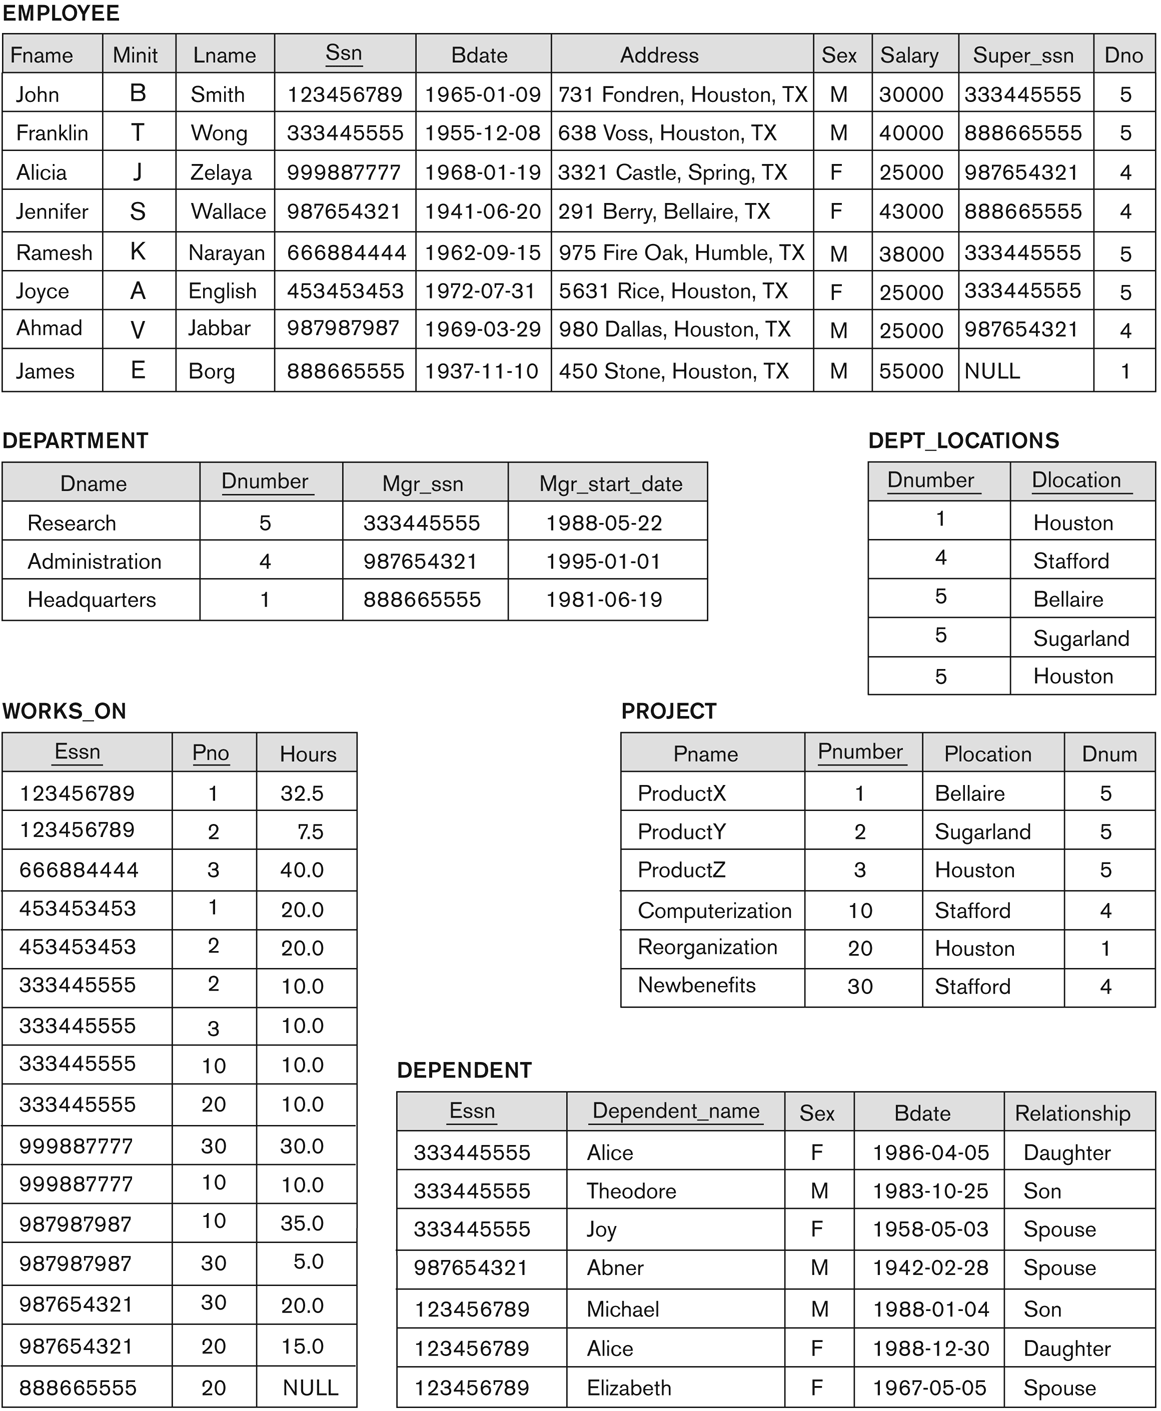
\includegraphics[width=\textwidth]{schema.png}
  \caption{Courtesy of Elmari\&Navathe's ``Fundamentals of Database systems
    -- 5\textsuperscript{th} edition'': relation schemas, representing a
    company business environment, and one of their possible conforming
    states.}
  \label{fig:schema}
\end{figure*}

% Roman numerals for in-text lists.
\makeatletter
\newcommand{\rmnum}[1]{\romannumeral #1}
\newcommand{\Rmnum}[1]{\expandafter\@slowromancap\romannumeral #1@}
\makeatother

% Automatic counter for example queries.
\newcounter{qcounter}
\newcommand{\Query}{\stepcounter{qcounter}(\theqcounter) }
\newcommand{\Queryd}{\stepcounter{qcounter}(\theqcounter$\ddagger$) }

Using the relation schemas outlined in figure~\ref{fig:schema}
page~\pageref{fig:schema}, build relational algebra queries satisfying the
following requests\footnote{`$\ddagger$'-marked requests were taken from
\cite{elmasri} example queries; the rest are the book's end-of-chapter
exercises.}: \Query~get employee tuples whose department number is 4.
\begin{flalign*}
  &\m{res} \lar \sigma_{Dno = 4}(\m{employee})&
\end{flalign*}

\Query Select employees whose salary is greater than $30,000\mathdollar$.
\begin{flalign*}
  &\m{res} \lar \sigma_{Salary > 30000}(\m{employee})&
\end{flalign*}

\Query Select employees who either work in department 4 and make over
$25,000\mathdollar$ per year, or work in department 5.
\begin{flalign*}
  &\sigma_{(Dno = 4 \band Salary > 25000) \bor Dno = 5}(\m{employee})&
\end{flalign*}

\Query List each employee's first and last name and salary.
\begin{flalign*}
  &\m{res} \lar \pi_{Fname, Lname, Salary}(\m{employee}) &
\end{flalign*}

\Query Retrieve first and last name of employees who work on department 1.
\begin{flalign*}
  &\m{res} \lar \pi_{Fname, Lname}(\sigma_{Dno = 1}(\m{employee})) &
\end{flalign*}

\Queryd Retrieve the social security number of all employees who work on
department 5 or who manage someone working on department 5.
\begin{flalign*}
  &\m{emp\_dep5} \lar \sigma_{Dno = 5}(\m{employee}) &\\
  &\m{emp\_ssn} \lar \pi_{Ssn}(\m{emp\_dep5}) &\\
  &\m{mgrs\_ssn} \lar \pi_{Super\_ssn}(\m{emp\_dep5}) &\\
  &\m{res} \lar \m{emp\_ssn} \cup \m{mgrs\_ssn} &
\end{flalign*}

\Query List the name of female employees dependents.
\begin{flalign*}
  &\m{fem\_emps} \lar \sigma_{Sex = F}(\m{employee}) &\db\\
  &\m{deps} \lar  \m{fem\_emps}\Join_{Essn = Ssn} \m{dependent} &\db\\
  &\m{res} \lar \pi_{Fname, Lname, Dependent\_name}(\m{deps}) &
\end{flalign*}

\Query Retrieve the name of the manager of each department.
\begin{flalign*}
  &\m{dep\_mgr} \lar \m{department} \Join_{Mgr\_ssn = Ssn} \m{employee} &\\
  &\m{res} \lar \pi_{Dname, Fname, Lname}(\m{dep\_mgr}) &
\end{flalign*}

\Query Retrieve the names of employees who work in \emph{any} of the projects
that ``John Smith'' works on.
\begin{flalign*}
  &\m{smith} \lar  \sigma_{Fname=John \land Lname=Smith}(\m{employee}) & \\
  &\m{smith\_pnos} \lar \pi_{Pno}(\m{smith} \Join_{Ssn = Essn} \m{works\_on})&\\
  &\m{emp\_ssn} \lar \pi_{Essn}(\m{smith\_pnos} * \m{works\_on})&\\
  &\m{smith\_ssn} \lar \pi_{Ssn}(\m{employee}) &\\
  &\m{res\_ssn(Ssn)} \lar \m{emp\_ssn}\ - \m{smith\_ssn} &\\
  &\m{res} \lar \pi_{Fname, Lname}(\m{employee} * \m{res\_ssn}) &
\end{flalign*}

\Queryd Retrieve the names of employees who work in \emph{all} of the
projects that ``John Smith'' works on.
\begin{flalign*}
  &\m{smith} \lar  \sigma_{Fname=John \land Lname=Smith}(\m{employee}) & \\
  &\m{smith\_pnos} \lar \pi_{Pno}(\m{smith} \Join_{Ssn = Essn} \m{works\_on})&\\
  &\m{all\_ssn\_pno} \lar \pi_{Essn, Pno}(works\_on) &\\
  &\m{emps\_ssn}(\m{Ssn}) \lar \m{all\_ssn\_pno} \div \m{smith\_pnos}&\\
  &\m{res} \lar \pi_{Fname, Lname}(\m{emps\_ssn} * \m{employee})&
\end{flalign*}

\Query For every male dependent, retrieve the dependent's name, and the
dependee employee name and department.
\begin{flalign*}
  &\m{male\_deps} \lar \sigma_{Sex=M}(\m{dependent}) &\\
  &\m{deps\_e} \lar \m{male\_deps} \Join_{Essn = Ssn} \m{employee} &\\
  &\m{deps\_e\_d} \lar \m{deps\_e} \Join_{Dno = Dnumber} \m{department} &\\
  &\m{res} \lar
    \pi_{\m{Dependent\_name}, \m{Fname}, \m{Lname}, \m{Dname}}(\m{deps\_e\_d})&
\end{flalign*}

\Query For all departments with employees, retrieve each department number,
the number of employees in the department, and their average salary. Rename
the result columns with meaningful names.
\begin{flalign*}
  &tmp \lar Dno\Im_{COUNT\ Ssn, AVERAGE\ Salary}(\m{emp}) &\\
  &\m{res}(\m{Dno}, \m{No\_of\_emps}, \m{avg\_salary}) \lar tmp &
\end{flalign*}

\Queryd Select all of the employees who are either directly supervised by
``James Borg'' or by any of his supervisees.
\begin{flalign*}
  &\m{borg} \lar \sigma_{Fname=James \land Lname=Borg}(\m{emp})&\\
  &\m{borg}(\m{Ssn0}) \lar \pi_{Ssn}(\m{borg}) &\\
  &\m{lvl1}(\m{Ssn1}) \lar \pi_{Ssn}(\m{borg} \Join_{Ssn0=Super\_ssn} \m{emp})&\\
  &\m{lvl2}(\m{Ssn2}) \lar \pi_{Ssn}(\m{lvl1} \Join_{Ssn1=Super\_ssn} \m{emp})&\\
  &\m{res} \lar (\rho_{(\m{Ssn})}(\m{lvl1} \cup \m{lvl2})) * \m{employee}&
\end{flalign*}

\Query Select names of department managers with at least one female
dependent.
\begin{flalign*}
  &\m{dept\_dep} \lar \m{department} \Join_{\m{Mgr\_ssn=Essn}} \m{dependent} &\\
  &\m{mgrs} \lar \sigma_{Sex = F}(\m{dept\_dep})&\\
  &\m{res} \lar \pi_{Fname, Lname}(\m{mgrs} \Join_{Essn = Ssn}\m{employee})&
\end{flalign*}

\Query Find employees who work on \emph{all} projects controlled by the
``Jennifer Wallace''-managed department.
\begin{flalign*}
  &\m{jennifer} \lar
    \sigma_{Fname = Jennifer \land Lname = Wallace}(\m{emp})&\\
  &\m{jen\_dep} \lar \m{jennifer} \Join_{Ssn = Mgr\_ssn} \m{department}&\\
  &\m{jen\_dep\_prj} \lar jen\_dep \Join_{Dnumber = Dnum} project&\\
  &\m{jen\_pnos}(\m{Pno}) \lar \pi_{Pnumber}(\m{jen\_dep\_prj})&\\
  &\m{ssn\_pno}(\m{Ssn, Pno}) \lar \pi_{Essn, Pno}(\m{works\_on})&\\
  &\m{emp\_ssn} \lar \m{ssn\_pno} \div \m{jen\_pnos}&\\
  &\m{res} \lar \pi_{Fname, Lname}(\m{emp\_ssn} * \m{employee})&
\end{flalign*}

\Query List names of employees working on two or more projects.
\begin{flalign*}
  &\m{tmp} \lar Essn\Im_{\m{COUNT}\ Pno}(\m{works\_on}) &\\
  &\m{prjs\_count}(\m{Ssn}, \m{Count}) \lar \m{tmp}&\\
  &\m{prjs\_2plus} \lar \sigma_{Count \ge 2}(\m{prjs\_count})&\\
  &\m{res} \lar \pi_{Fname, Lname}(prjs\_2plus * employee)&
\end{flalign*}

\Query Retrieve the names of all employees on department $5$ who work more
than $10$ hours per week on the project `ProductX'.
\begin{flalign*}
  &\m{e\_w} \lar \m{employee} \Join_{Ssn = Essn} \m{works\_on}&\\
  &\m{e\_w\_p} \lar \m{e\_w} \Join_{Pno = Pnumber} \m{project}&\\
  &\m{res} \lar
    \sigma_{Dno = 5 \ \land\ hours > 10\ \land\ Pname=ProductX}(e\_w\_p)&
\end{flalign*}

\Query List the names of all employees who have the same dependent name as
themselves.
\begin{flalign*}
  &\m{e\_d} \lar (\m{employee} \Join_{Ssn = Essn} \m{dependent})&\\
  &\m{emps} \lar \sigma_{Fname = Dependent\_name}(e\_d)&\\
  &\m{res} \lar \pi_{Fname, Lname}(\m{emps})&
\end{flalign*}

\Query For each project, list the project name and the total hours per week
(by all employees) spent on the project.\footnote{The answer assumes there's
at least one employee per project.}
\begin{flalign*}
  &\m{tmp} \lar Pno\Im_{SUM\ Hours}(works\_on)&\\
  &\m{prj\_hours}(\m{Pnumber}, \m{Total}) \lar \m{tmp}&\\
  &\m{res} \lar \pi_{Pname, Total}(\m{prj\_hours} * \m{project})&
\end{flalign*}

\Query Retrieve the names of employees who work on \emph{every} company
project.
\begin{flalign*}
  &\m{all\_pnos}(\m{Pno}) \lar  \pi_{Pnumber}(project)&\\
  &\m{ssn\_pnos}(\m{Ssn}, \m{Pno}) \lar \pi_{Essn, Pno}(works\_on)&\\
  &\m{ssn} \lar \m{ssn\_pnos} \div \m{all\_pnos} &\\
  &\m{res} \lar \pi_{Fname, Lname}(ssn * employee)&
\end{flalign*}

\Query Retrieve the names of all employees who do not work on \emph{any}
project.
\begin{flalign*}
  &\m{all\_ssn} \lar \pi_{Ssn}(\m{employee})&\\
  &\m{working\_ssn}(Ssn) \lar \pi_{Essn}(\m{works\_on})&\\
  &\m{free\_ssn} \lar \m{all\_ssn} - \m{working\_ssn}&\\
  &\m{res} \lar \pi_{Fname, Lname}(\m{free\_ssn} * \m{employee})&
\end{flalign*}

\Query Retrieve the average salary of all female employees.
\begin{flalign*}
  &\m{res} \lar \Im_{\m{AVERAGE}\ Salary}(\sigma_{Sex=F}(employee))&
\end{flalign*}

%% Note: when applying aggregate functions to a particular column,
%% its NULL values are discarded.
\Query For each department, retrieve the department name and the average
salary of all of its employees.\footnote{Due to a typesetting limitation,
we've used the non-standard symbol `$\lhd$' to denote a \emph{left outer
join}.}
\begin{flalign*}
  &\m{tmp} \lar \m{Dno}\Im_{\m{AVERAGE}\ Salary}(employee)&\\
  &\m{deps\_avg}(Dno, Avg\_salary) \lar \m{tmp}&\\
  &\m{deps} \lar \m{department} \lhd_{Dnumber = Dno} \m{deps\_avg}&\\
  &\m{res} \lar \pi_{Dname, Avg\_salary}(\m{deps})&
\end{flalign*}

\Query List the names of all department managers who have no dependents.
\begin{flalign*}
  &\m{dept\_dep} \lar \m{department} \Join_{\m{Mgr\_ssn = Essn}} \m{dependent}&\\
  &\m{mgrs\_dep}(\m{Ssn}) \lar \pi_{Essn}(\m{dept\_dep})&\\
  &\m{all\_mgrs}(\m{Ssn}) \lar \pi_{Mgr\_ssn}(\m{department})&\\
  &\m{mgrs\_no\_dep} \lar \m{all\_mgrs} - \m{mgrs\_dep}&\\
  &\m{res} \lar \pi_{Fname, Lname}(\m{mgrs\_no\_dep} * \m{employee})&
\end{flalign*}

\Query Find the names and addresses of all employees who work on at least one
project located in Houston, but whose department has no location in
Houston.\newline
\emph{Answer}: the solution can be divided to three parts;
\rmnum{1}) employees who work on at least one project in Houston:
\begin{flalign*}
  &\m{e\_w} \lar \m{employee} \Join_{Ssn = Essn} \m{works\_on}&\\
  &\m{e\_w\_p} \lar \m{e\_w} \Join_{Pno = Pnumber} \m{project}&\\
  &\m{houston\_ssn} \lar \pi_{Ssn}(\sigma_{Plocation = Houston}(\m{e\_w\_p}))&
\end{flalign*}
\rmnum{2}) employees whose department has no location in Houston:
\begin{flalign*}
  &\m{houston\_deps} \lar \sigma_{Dlocation = Houston}(dept\_locations)&\db\\
  &\m{houston\_dno}(\m{Dnum}) \lar \pi_{Dnumber}(houston\_deps)&\db\\
  &\m{all\_dno}(\m{Dnum}) \lar \pi_{Dnumber}(department)&\db\\
  &\m{no\_houston\_dno} \lar \m{all\_dno} - \m{houston\_dno}&\db\\
  &\m{tmp} \lar \m{employee} \Join_{\m{Dno = Dnum}} {no\_houston\_dno}&\\
  &\m{no\_houston\_dept\_ssn} \lar \pi_{Ssn}(\m{tmp})&
\end{flalign*}
\rmnum{3}) final result: common employees from the two queries above,
satisfying the original request.
\begin{flalign*}
  &\m \m{common} \lar \m{houston\_ssn} \cap \m{no\_houston\_dept\_ssn}&\\
  &\m{res} \lar \pi_{Fname, Lname, Address}(\m{common} * \m{employee})&
\end{flalign*}

%%
%% [*] A section discussing relational algerba's recursive closure
%% infeasibility should be included. A proof of this inability should
%% also be included, possibly the one done by Alfred Aho and Jeffery
%% Ullman's in `Universality of Data Retrieval Languages'.
%%

\begin{thebibliography}{3}
\bibitem{codd-v1}
  E. F. Codd,
  \emph{A Relational Model of Data for Large Shared Data Banks}.
  Communications of the ACM, Volume 13, Issue 6, June 1970.

\bibitem{codd-semantic}
  E. F. Codd,
  \emph{Extending the data base relational model to capture more meaning}.
  ACM Transactions on Database Systems, Volume 4, Issue 4, December 1979.

\bibitem{codd-v2}
  E. F. Codd,
  \emph{Relational Model for Database Management -- version 2}.
  Addison-Wesley, 1990.

\bibitem{elmasri}
  RA. Elmasri \& S. B. Navathe,
  \emph{Fundamentals of Database Systems -- 5\textsuperscript{th} Edition}.
  Addison-Wesley, 2007.
\end{thebibliography}

\begin{center}\small{Typeset with \LaTeX}\end{center}

\end{document}
